\section*{Problem 2: Encoding categorical variables}

\paragraph{(a) Cardinality and preparation.} The retail data contain 397,924 transactions, with no missing values in the supplied columns.
\begin{center}
\begin{tabular}{lrrr}
\toprule
Feature & Unique values & Unique in training & Singleton categories\\
\midrule
StockCode & 3,665 & 3,595 & 167\\
CustomerID & 4,339 & 4,311 & 72\\
\bottomrule
\end{tabular}
\end{center}
One-hot encoding would have 8,004 columns and only two nonzero entries per row. A dense float32 matrix for the full dataset would require about 11.86 GiB, so it is inefficient. Sparse one-hot encoding is feasible. Target encoding gives two numerical features, while embeddings provide compact learned category representations.

I use a random 70/15/15 split with seed 42: 278,546 training, 59,689 validation, and 59,689 test observations. Category vocabularies, encodings, and preprocessing statistics are learned from training data. Only validation loss controls early stopping.

Quantity is strongly right-skewed: the median is 6, mean 13.02, 99th percentile 120, and maximum 80,995. I train all three models with squared error on $z=\log(1+Y)$:
\[
L=\frac1n\sum_i\big(z_i-\widehat z_i\big)^2.
\]
This reduces the influence of enormous orders. I predict $\widehat Y=\max\{1,\exp(\widehat z)-1\}$ and report log-space MSE, its square root (RMSLE), and raw-scale MAE/RMSE. The inverse-transformed prediction targets log-space accuracy; it is not generally the arithmetic conditional mean of Quantity.

\paragraph{(b) Target encoding.} For each feature separately, I compute a smoothed arithmetic mean of raw Quantity:
\[
\operatorname{TE}(c)=\frac{\sum_{i:X_i=c}Y_i+20\overline Y}{n_c+20},
\]
where $\overline Y$ and $n_c$ are computed from the relevant training portion. Each training row receives a five-fold out-of-fold encoding, excluding every target in its own fold. Validation and test use maps fitted on the entire training split. Unseen categories receive the global training mean. This prevents a row's target from leaking into its own input.

I apply $\log(1+\operatorname{TE})$ and standardize the two inputs using the out-of-fold training statistics. A $2\to64\to32\to1$ ReLU network predicts $z$. Its selected checkpoint is epoch 13, giving test log MSE $0.402013$ and RMSLE $0.634045$.

\paragraph{(c) Embedding model.} Each feature has its own 16-dimensional trainable embedding. Their concatenation feeds a $32\to64\to32\to1$ ReLU network. Categories are assigned indices using training data only; unseen categories use a fixed zero vector. The test set has 51 rows with unseen StockCodes and 16 with unseen CustomerIDs, possibly overlapping. The selected checkpoint is epoch 23. Test log MSE is $0.268072$ and RMSLE is $0.517756$, improving log MSE by about $33.3\%$ over target encoding.

\newpage
\paragraph{(d) Combined model.} I concatenate the two target-encoded inputs and the 32 embedding coordinates, then fit a $34\to64\to32\to1$ ReLU network. It uses the same out-of-fold training encodings as part (b). All three networks use Adam, learning rate $0.003$, weight decay $10^{-4}$, batch size 2,048, at most 40 epochs, and patience 6. Each restores its best validation checkpoint; the hybrid selects epoch 18.

\begin{center}
\small
\begin{tabular}{lrrrrr}
\toprule
Model & Val. log MSE & Test log MSE & Test RMSLE & Test MAE & Test RMSE\\
\midrule
Constant & 1.010325 & 0.996641 & 0.998319 & 10.2061 & 41.3628\\
Target encoding & 0.400340 & 0.402013 & 0.634045 & 6.9660 & 32.3021\\
Embeddings & 0.267290 & \textbf{0.268072} & \textbf{0.517756} & \textbf{5.7792} & 30.4097\\
Combined & \textbf{0.264604} & 0.268360 & 0.518035 & 5.8948 & \textbf{29.6528}\\
\bottomrule
\end{tabular}
\end{center}
The constant baseline predicts the training mean of $z$, then applies the same inverse transform. All reported test values use the untouched test split. The combined model has the lowest validation error, but embeddings alone are slightly better on test log MSE. The test difference is only $0.000288$, so there is no clear gain from combining them on the primary metric. The combined model has the lowest raw RMSE, showing that the ranking depends on the metric.

\begin{figure}[H]
\centering
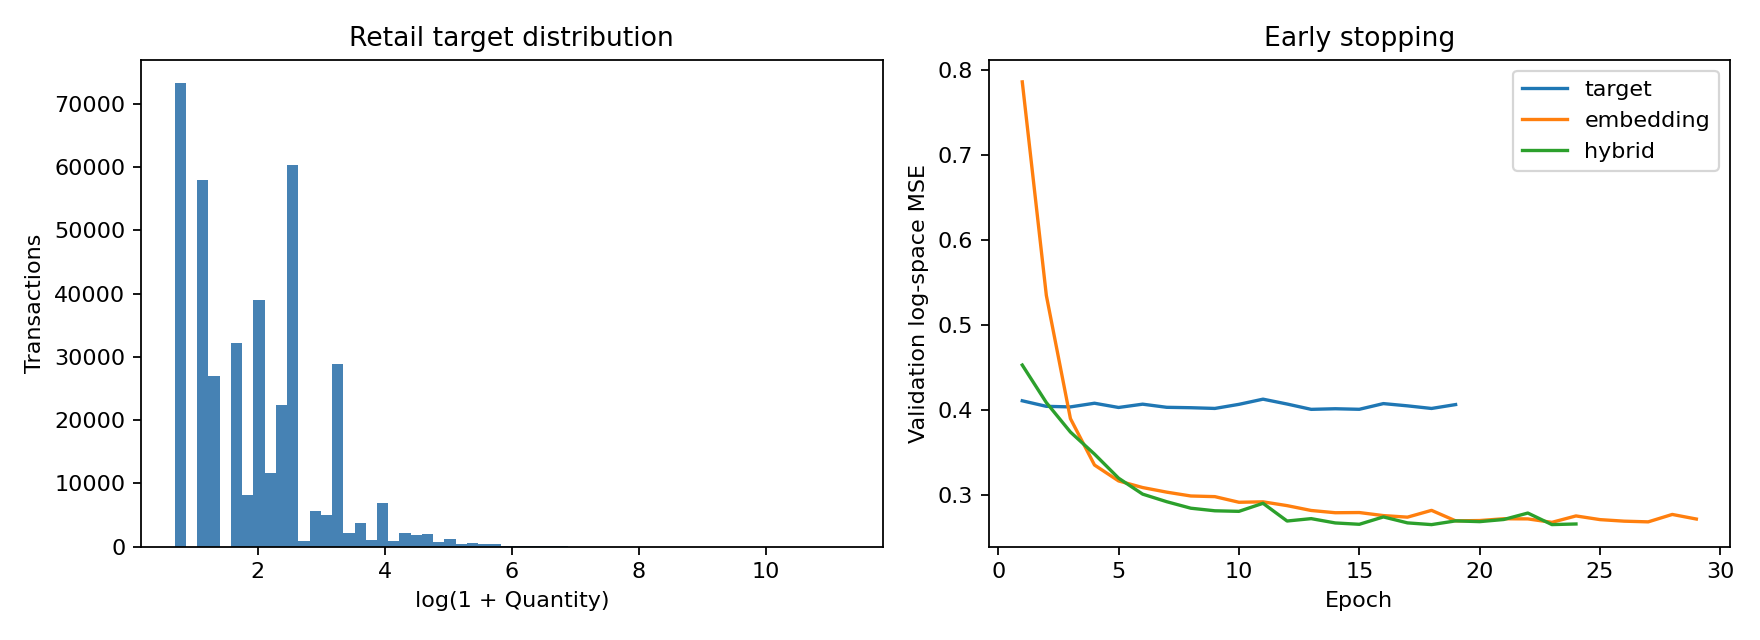
\includegraphics[width=\textwidth]{images/problem2/retail_results.png}
\caption{The transformed retail target and validation learning curves. The selected checkpoints precede the end of each curve.}
\end{figure}

\paragraph{(e) Interpretation.} Target encoding collapses each category into one average. Two products with the same average order size become indistinguishable under this encoding, even if they interact differently with individual customers. An embedding gives each category several coordinates, learned jointly with the prediction network. The network can use these coordinates to represent useful category properties and nonlinear customer--product interactions.

The much lower test error of the embedding model suggests that category-specific information beyond two marginal means is useful here. The combined model supplies both summary statistics and learned representations, but some of this information is redundant. Its small validation improvement does not translate into a clear improvement in test RMSLE.

This random transaction split primarily evaluates customers and products already seen during training. It does not establish performance for entirely new customers/products or future time periods. The results come from one split and seed, so the tiny difference between embeddings and the combined model should not be treated as statistically established.
